\chapter{线性映射矩阵表示(II)}

可逆性是矩阵的一个重要性质,我们将在本节讨论矩阵的可逆性及其运算性质. 除此之外,我们还会介绍积空间和商空间,以及其上定义的线性映射和矩阵表示作为综合应用,特别是商空间能给我们一定的启示并且在未来更深入的数学学习中非常重要.

\section{矩阵的逆}

\subsection{基本概念}

要引入矩阵的逆的概念,我们需要首先讨论线性映射的逆. 我们这里给出线性映射的逆的定义:
\begin{definition}[线性映射的逆] \label{def:8:可逆映射} \index{ni@逆 (inverse)}
    设$\sigma \in \mathcal{L}(V_1,V_2)$. 若存在$\tau \in \mathcal{L}(V_2,V_1)$使得$\sigma \tau = I_{V_2}$且$\tau \sigma = I_{V_1}$,则称$\sigma$\term{可逆}\index{ni!ke@可逆 (invertible)},并称$\tau$为$\sigma$的逆映射\index{ni!yingshe@映射 (inverse map)}.
\end{definition}
其中$I_{V_1}$和$I_{V_2}$分别是$V_1$和$V_2$上的恒等映射.

在之前有关线性映射基本定理的讨论中,我们提到了双射的概念. 事实上,在映射的语境下,双射与可逆是完全等价的. 我们有如下定理:
\begin{theorem}
    设$\sigma \in \mathcal{L}(V_1,V_2)$,则$\sigma$可逆$\iff \sigma$是双射.
\end{theorem}

因此在本讲义的语境下,双射与可逆是完全等价的. 关于这一定理我们有如下说明:
\begin{enumerate}
    \item 定理证明不属于本讲义需要覆盖的内容,相信一般的微积分或数学分析教材都会涉及;

    \item 这一定理事实上不一定针对线性映射,对于函数而言也有双射与可逆等价,只是在函数的语境下逆映射被称为反函数;

    \item 由于双射要求单射和满射,而单射性与核空间维数为0等价,由线性映射基本定理,双射应有出发空间维数等于像空间维数,而满射性要求像空间维数等于到达空间维数,因此双射要求出发空间和到达空间必须维数相同.
\end{enumerate}

在\autoref{def:8:可逆映射} 的语境下,我们取$V_1$的一组基$B_1=\{\alpha_1,\alpha_2,\ldots,\alpha_n\}$,$V_2$的一组基$B_2=\{\beta_1,\beta_2,\ldots,\beta_n\}$(特别注意根据我们上述讨论两个空间维数一致),则$\sigma$关于$B_1$和$B_2$的矩阵为$A=(a_{ij})_{m \times n}$,$\tau$关于$B_2$和$B_1$的矩阵为$B=(b_{ij})_{n \times m}$.

我们知道线性映射的复合对应矩阵乘法,因此$\tau\sigma:V_1\to V_1$关于$V_1$的基$B_1$和$\sigma\tau:V_2\to V_2$关于$V_2$的基$B_2$对应的矩阵分别为$BA$和$AB$,而我们很容易证明恒等映射关于任何基的矩阵均为单位矩阵,因此我们有$BA=E$和$AB=E$. 由此我们从可逆映射的角度引入矩阵的逆的概念:
\begin{definition}[矩阵的逆]
    设$A \in \mathbf{M}_n(\mathbf{F})$. 若存在$B \in \mathbf{M}_n(\mathbf{F})$使得$AB=BA=E$,则称矩阵$A$可逆,并把$B$称为$A$的\term{逆矩阵}\index{ni!juzhen@矩阵 (inverse matrix)},记作 $ B = A^{-1} $.
\end{definition}
在一些比较经典的教材中可逆矩阵也被称为非奇异矩阵,不可逆矩阵被称为\term{奇异矩阵}\index{qiyijuzhen@奇异矩阵 (singular matrix)}.

注意,逆矩阵定义基于方阵,非方阵没有上述逆矩阵. 广义逆矩阵允许非方阵,但那是另一个定义,我们不需要掌握. 对于可逆矩阵,注意以下两个定理:
\begin{theorem}
    可逆矩阵$A$的逆矩阵唯一.
\end{theorem}

\begin{theorem}
    设$A,B\in \mathbf{M}_n(\mathbf{F})$,则$AB=E \iff A$与$B$互为逆矩阵(即对于方阵而言,$AB=E\iff BA=E\iff A,B$可逆).
\end{theorem}
这两个定理的证明见教材130页. 特别注意唯一性的证明,我们在证明群的单位元唯一时使用了完全一致的思想,请务必掌握.

\subsection{基本性质}

\begin{enumerate}[label=(\arabic*)]
    \item 主对角元都是非零数的对角矩阵一定可逆,且逆矩阵就是对角线上元素取倒数(单位矩阵即为特例,其逆矩阵是其自身);

    \item \label{item:8:逆矩阵性质:2}
          注意没有加法性质(例如$A$可逆(则$-A$也可逆),但$A+(-A)=O$不可逆),对于数乘有$(\lambda A)^{-1}=\lambda^{-1}A^{-1}$;

    \item \label{item:8:逆矩阵性质:3}
          $(AB)^{-1}=B^{-1}A^{-1},\enspace (A_1A_2\cdots A_k)^{-1}=A_k^{-1}\cdots A_2^{-1}A_1^{-1}$;注意这一点和 \ref*{item:8:逆矩阵性质:2} 的证明都只需要直接验证结果即可,即因为$ABB^{-1}A^{-1}=AA^{-1}=E$,所以根据逆的唯一性可知$(AB)^{-1}=B^{-1}A^{-1}$一定成立;

    \item $(A^k)^{-1}=(A^{-1})^k,\enspace A^kA^m=A^{k+m},\enspace (A^k)^m=A^{km}$;注意这里的$k$和$m$不一定需要非负,事实上负数就是逆矩阵的幂次或幂次的逆,如$A^{-2}=(A^{-1})^2=(A^2)^{-1}$;

    \item 若$A$和$B$可逆,则$A\neq O$且$B\neq O$能推出$AB\neq O$,并且$A$可逆且$AB=O$可以推出$B=O$. 除此之外还有消去律成立,即$A \neq O$则有$AB=AC \implies B=C$成立.
\end{enumerate}

\subsection{逆矩阵的求解(基本方法I)}

在介绍完性质后我们非常关心如何给定一个具体的矩阵求出它的逆的问题,这里我们给出第一种基本方法,即基于解方程的方法.

事实上,我们在矩阵乘法一节中就将$AX=b$和$\sigma(a)=b$联系在一起,其中$\sigma$在某组基下表示矩阵为$A$. 回顾本讲开头引入可逆矩阵的过程,可逆矩阵$A$应当是可逆线性映射$\sigma$关于某组基的表示矩阵. 对于可逆映射而言,首先必须是单射,因此$\sigma(a)=b$只能有唯一解,因此$AX=b$只能有唯一解.

事实上我们可以很简便地表达出这个解. 我们在$AX=b$左右同时左乘$A^{-1}$(矩阵乘法不可交换所以必须在同一侧乘),有$A^{-1}AX=A^{-1}b$,即$X=A^{-1}b$.

因此,当$A$可逆时,对于任意的$b$线性方程组都有唯一解,且解可以被表示为$X=A^{-1}b$的形式. 因此我们可以通过解线性方程组的方法求解逆矩阵. 我们将通过下面这个例子详细介绍这种方法的计算过程:
\begin{example}
    用上述方法求矩阵$A=\begin{pmatrix}1 & -1 & 1 \\ 0 & 1 & 2 \\ 1 & 0 & 4\end{pmatrix}$的逆矩阵.
\end{example}

\begin{solution}
    见教材132页例3.
\end{solution}

关于逆矩阵的求解问题,我们将在介绍完初等变换后介绍第二种基本方法,剩余的进阶解法将在\hyperref[chap:矩阵运算进阶(II)]{矩阵运算进阶(II)}中介绍更多手段,以及我们会介绍矩阵方程求解的方法. 本节我们囿于一些计算技巧和基本概念暂未引入所以无法完全展开这些技巧.

\subsection{广义逆矩阵}

在本节开头我们提到,逆矩阵是基于方阵定义的. 对于非方阵而言,我们有如下广义逆的定义,当然不要求读者在这门课中掌握. 对于每一个$m \times n$阶矩阵$A$,都存在唯一的$n \times m$阶矩阵$X$,使得:
\begin{enumerate}
    \item $AXA=A$;

    \item $XAX=X$;

    \item $AX$和$XA$均为共轭对称矩阵.
\end{enumerate}
我们称$X$为矩阵$A$的Moore-Penrose广义逆矩阵,记作$M=A^\dagger$. 此处不赘述其证明和算法,感兴趣的同学可以自行查阅相关资料. 我们可以从两个角度认识这一定义,首先是取$A$为可逆矩阵,发现此定义是相容的,其次是通过这一矩阵可以获得线性方程组$AX=b$最小二乘解$X=A^\dagger b$. 广义逆矩阵在各个领域的研究中应用很广泛,所以在此提一下它的概念.

\section{线性空间的积}

接下来的两节我们将综合应用之前所学习的基本知识,介绍两个重要的线性空间,即积空间和商空间,以及其上定义的线性映射. 在这两节中我们将完整地展示从定义的引入开始,如何研究一个线性空间,如何合理定义线性映射,如何应用前述知识综合地给出一些空间和映射的性质,这对于我们是一个重要的思维训练.

\subsection{线性空间的积的定义与性质研究}

我们首先探讨线性空间的积,或者积空间. 熟知集合有笛卡尔积运算,而线性空间是定义在集合上的代数结构,因此我们有一个自然的问题,即我们能否在多个线性空间的对应的集合的笛卡尔积上定义加法和数乘运算,使其成为一个线性空间?

答案是肯定的,但我们需要首先声明的一点是,构成笛卡尔积的这些线性空间必须定义在同一个数域上,否则新集合上的数乘我们将很难定义,因为数域不同我们将很难选择数乘的常数应该选择来自于哪个线性空间的数域.
\begin{definition}\label{def:8:积空间}
    设$V_1,V_2,\ldots,V_n$是数域$\mathbf{F}$上的线性空间,我们有如下三个定义:
    \begin{enumerate}
        \item 线性空间的积:
              \[V_1 \times V_2 \times \cdots \times V_n=\{(v_1,v_2,\ldots,v_n)\mid v_i \in V_i,\enspace i=1,2,\ldots,n\};\]

        \item 规定$V_1 \times V_2 \times \cdots \times V_n$上加法和数乘运算:
              \begin{enumerate}
                  \item 加法:$(v_1,v_2,\ldots,v_n)+(u_1,u_2,\ldots,u_n)=(v_1+u_1,v_2+u_2,\ldots,v_n+u_n)$;

                  \item 数乘:$\lambda(v_1,v_2,\ldots,v_n)=(\lambda v_1,\lambda v_2,\ldots,\lambda v_n)$.
              \end{enumerate}
    \end{enumerate}
\end{definition}

事实上我们很容易验证上述定义的线性空间的积在定义的加法和数乘运算下构成线性空间,我们将放在习题中供读者练习. 接下来我们要研究这一线性空间的性质. 事实上,我们早在有限维线性空间一节中就说明了,一个线性空间的核心结构就是其基和维数,因此我们首先研究它们. 事实上,对于积空间,它的基和维数的确定是非常符合我们的直觉的,我们来看一个例子:
\begin{example}
    求积空间$\mathbf{R}[x]_3\times\mathbf{R}^2$的一组基.
\end{example}

\begin{solution}
    我们知道$\mathbf{R}[x]_3$的一组基为$1,x,x^2$,而$\mathbf{R}^2$的一组基为$(1,0),(0,1)$. 很自然的想法是:我们可以先取$\mathbf{R}[x]_3$的一组基,$\mathbf{R}^2$的位置置零,然后反之取$\mathbf{R}^2$的一组基,$\mathbf{R}[x]_3$的位置置零,即$(1,(0,0)),\ (x,(0,0)),\ (x^2,(0,0)),\ (0,(1,0)),\ (0,(0,1))$. 我们很容易可以证明上述向量组满足基的两个条件:线性无关和张成空间.
\end{solution}

上述例子中的基的构造方法是很自然的,而且我们会发现,在这样取基的情况下积空间的维数很显然就是各个线性空间的维数之和. 我们可以很容易地推广到一般情况:
\begin{theorem}\label{thm:8:积空间维数}
    设$V_1,V_2,\ldots,V_n$是数域$\mathbf{F}$上的有限维线性空间,则$V_1 \times V_2 \times \cdots \times V_n$是有限维线性空间,且
    \[\dim(V_1 \times V_2 \times \cdots \times V_n)=\dim V_1+\dim V_2+\cdots+\dim V_n.\]
\end{theorem}

\begin{proof}
    我们取$V_i$的一组基,对这组基中每个向量,我们取$V_1 \times V_2 \times \cdots \times V_n$中的这样的向量:其中第$j$个位置为此向量,其余位置为零向量,这样我们遍历所有$V_i$和每个$V_i$的基向量我们就得到了$V_1 \times V_2 \times \cdots \times V_n$的一组基(线性无关和张成性是很容易验证的),这组基的长度(即维数)为$\dim V_1+\dim V_2+\cdots+\dim V_n$.
\end{proof}

\subsection{线性空间的积与直和}

本节我们将通过线性空间的积的角度来讨论直和的维数特点. 事实上,我们的手段就是构造线性映射,然后利用线性映射基本定理来得到结论.
\begin{theorem}\label{thm:8:积与直和}
    设$U_1,U_2,\ldots,U_n$是$V$的子空间,我们定义线性映射$\sigma:U_1 \times U_2 \times \cdots \times U_n \to U_1+U_2+\cdots+U_n$,使得$\sigma(u_1,u_2,\ldots,u_n)=u_1+u_2+\cdots+u_n$,则$U_1+U_2+\cdots+U_n$是$V$的直和$\iff \sigma$是双射.
\end{theorem}

\begin{proof}
    \begin{enumerate}
        \item 充分性:设$\sigma$是双射,则$\sigma$首先是单射. 根据单射的等价条件,我们有$\ker \sigma=\{0\}$,即$u_1+u_2+\cdots+u_n=0$必须有$u_1=u_2=\cdots=u_n=0$,而这正是\autoref{thm:4:直和等价命题} 中直和的等价条件;

        \item 必要性:设$U_1+U_2+\cdots+U_n$是直和,我们证明$\sigma$是单的、满的:
              \begin{enumerate}
                  \item 单射:设$\sigma(u_1,u_2,\ldots,u_n)=0$,即$u_1+u_2+\cdots+u_n=0$,由直和的等价条件可知$u_1=u_2=\cdots=u_n=0$,即$\sigma$的核空间只有出发空间零元,故是单射;

                  \item 满射:实际上是由这个线性映射的定义直接保证的. $\forall u \in U_1+U_2+\cdots+U_n$,根据和的定义一定有分解$u=u_1+u_2+\cdots+u_n$,其中$u_i \in U_i$,因此根据$\sigma$的定义$\sigma(u_1,u_2,\ldots,u_n)=u$,即任意$u$我们都可找到原像,故是满射.
              \end{enumerate}
    \end{enumerate}
\end{proof}

事实上在证明中我们看到,$\sigma$的定义保证了其满射性,因此定理中最后的双射改为单射也是统一的. 通过这一定理我们可以直接得出以下结论:
\begin{theorem}
    设$U_1,U_2,\ldots,U_n$是有限维线性空间$V$的子空间,则$U_1+U_2+\cdots+U_n$是$V$的直和$\iff \dim(U_1+U_2+\cdots+U_n)=\dim U_1+\dim U_2+\cdots+\dim U_n$.
\end{theorem}

\begin{proof}
    根据\autoref{thm:8:积与直和},$U_1+U_2+\cdots+U_n$是$V$的直和$\iff \sigma$是双射. 我们很容易验证$\sigma$是线性映射,而线性双射我们又称同构映射,同构映射的出发空间和到达空间维数相等,因此$\sigma$是双射$\iff \dim(U_1 \times U_2 \times \cdots \times U_n)=\dim(U_1+U_2+\cdots+U_n)$,最后根据\autoref{thm:8:积空间维数} 积空间的维数可知定理成立.
\end{proof}

这里我们用同构映射完成证明,如果对同构不熟悉的可以回顾定义和等价条件,或者自己用线性映射基本定理进行推导. 由此,我们通过在积空间上定义映射,结合\hyperref[thm:6:线性映射基本定理]{线性映射基本定理}(或同构)得到了\autoref{thm:4:直和等价命题} 中关于维数的命题. 总结而言,在积空间的讨论中我们展现了一个比较完整地学习路径:从定义积空间的想法(来源于集合的笛卡尔积),到如何自然地定义出这一空间的加法和数乘运算,然后研究构造出的空间的基本结构有什么特点,然后进一步构造其上线性映射,得到一些其他的结论. 这一路径的每一步都是非常自然的,而且是学习一个数学概念的常见思路,希望读者不仅是在线性代数中体会到这种学习路径,在其他数学课甚至其他学科中都能总结出这样一条引入—定义—性质—应用的自然路径.

最后我们再看一个拓展的问题,我们希望进一步看到构造同构映射带来的研究问题的方便性:
\begin{example}
    设$V_1,V_2,\ldots,V_n,W$是数域$\mathbf{F}$上的线性空间,证明:$\mathcal{L}(V_1 \times V_2 \times \cdots \times V_n,W)$与$\mathcal{L}(V_1,W) \times \mathcal{L}(V_2,W) \times \cdots \times \mathcal{L}(V_n,W)$同构.
\end{example}
有的读者可能看见这题就会觉得非常简单,因为有限维线性空间的前提下二者维数显然相同,然而我们这里并未限定有限维线性空间,因此需要读者自己构造同构映射.

\begin{solution}
    $\forall f\in \mathcal{L}(V_1 \times V_2 \times \cdots \times V_n,W)$,我们定义$f_i:V_i\to W(i=1,2,\ldots,m)$满足
    \[f_i(v_i)=f(0,\ldots,0,v_i,0,\ldots,0),\]
    其中$v_i$位于第$i$个位置,其余位置为零向量.

    定义$\varphi:\mathcal{L}(V_1 \times V_2 \times \cdots \times V_n,W)\to \mathcal{L}(V_1,W) \times \mathcal{L}(V_2,W) \times \cdots \times \mathcal{L}(V_n,W)$,使得$\varphi(f)=(f_1,f_2,\ldots,f_m)$,则接下来我们要验证$\varphi$就是我们要求的同构映射.
\end{solution}

\section{线性空间的商}

\subsection{商空间的引入与仿射子集}

我们继续循着数学概念学习的自然路径,再来审视一个新的概念——商空间. 在第一讲中我们描述了一个非常重要的概念——等价类. 我们希望在一个线性空间$V$中构造等价类组成商集,并在商集中引入加法和数乘运算,使得商集构成线性空间,这便是本节要讨论的商空间的来由. 总结一下,我们这里有两个需求:其一是构造合适的等价关系,其二是构造合理的加法和数乘运算.

回忆集合的等价关系的建立,都是元素之间的关系. 例如等于关系是实数集合中的实数之间的关系,因此要在线性空间中建立等价关系,我们需要考虑两个元素(即向量)的关系. 我们可以考虑$V$的子空间$U$,并将关系$R$定义为
\[\forall\alpha,\beta\in V,\enspace\alpha\,R\,\beta\iff \alpha-\beta\in U.\]
即两个向量的差向量在一个规定的子空间中时称它们等价. 我们会很容易地验证出这个关系就是等价关系:
\begin{enumerate}
    \item (自反性) $\forall \alpha\in V,\enspace\alpha-\alpha=0\in U$,故$\alpha\,R\,\alpha$;

    \item (对称性) $\forall \alpha,\beta\in V,\enspace\alpha\,R\,\beta\implies \alpha-\beta\in U\implies \beta-\alpha=-(\alpha-\beta)\in U\implies \beta\,R\,\alpha$;

    \item (传递性) $\forall \alpha,\beta,\gamma\in V,\enspace\alpha\,R\,\beta,\enspace\beta\,R\,\gamma\implies \alpha-\beta\in U,\enspace\beta-\gamma\in U\implies \alpha-\gamma=(\alpha-\beta)+(\beta-\gamma)\in U\implies \alpha\,R\,\gamma$.
\end{enumerate}
证明只用到了线性空间的加法单位元、逆元性质且运算封闭. 接下来我们可以基于此定义这一等价关系的等价类:
\[\overline{\alpha}=\{\beta\in V \mid \beta\,R\,\alpha\}=\{\beta\in V \mid \beta-\alpha\in U\}=\{\beta\in V \mid \beta=\alpha+\gamma,\enspace\gamma\in U\}\]
最后一个集合还可以进一步写成$\{\alpha+\gamma \mid \gamma\in U\}$,我们记为$\alpha+U$,称之为$V$的仿射子集. 我们给出如下完整的定义:
\begin{definition}[仿射子集] \index{fangsheziji@仿射子集 (affine subset)}
    设$v\in V$,$U$是$V$的子空间,则$V$的\term{仿射子集}是$V$的形如$v+U$的子集,其中$v+U$定义为
    \[v+U=\{v+u \mid u\in U\}.\]
\end{definition}
根据我们之前的讨论,仿射子集就是我们在线性空间上定义的等价关系的等价类. 基于等价类的性质,我们有如下定理:
\begin{theorem}
    设$U$是$V$的子空间,$v,w\in V$,则以下陈述等价:
    \begin{enumerate}
        \item $v-w\in U$;

        \item $v+U=w+U$;

        \item $(v+U)\cap(w+U)\neq \varnothing$.
    \end{enumerate}
\end{theorem}

还需要强调的一点是,$(v+U)+(w+U)$与$(v+w)+U$是完全相同的集合,等价性是显然的,我们只需要展开写出仿射子集定义然后证明两个集合互相包含即可. 当然更一般的情形为
\[(v_1+U_1)+(v_2+U_2)+\cdots+(v_n+U_n)=(v_1+v_2+\cdots+v_n)+U_1+U_2+\cdots+U_n.\]

按照我们之前所说的学习数学的基本思路,在学习一个新的概念后我们会尝试考察它是否具有某些特别的性质,从而可以更深入地理解这一概念. 类似于线性空间我们介绍过原点的直线、平面然后介绍一般线性空间的基本结构是基和维数,我们从直观入手,然后逐步考察仿射子集的基本结构.

相信读者对``仿射''一词并不完全陌生,仿射变换实际上就是形如\[\vec{y}=A\vec{x}+\vec{b}\]的映射,其中$\vec{y},\vec{x},\vec{b}$为向量,$A$是一个矩阵. 实际上一元向量的情况就对应着一条斜率为$A$截距为$b$的直线.

事实上,若$V$为二维空间(平面),$U$为$V$的一维子空间,则其几何意义就是一条过原点的直线,而集合$v+U$实际上将原集合所有点沿着$v$的方向平移,可以得到截距不为0的直线,这就体现了``仿射''一词的意义. 高维空间则是同理,只是我们很难直观地看到这一点. 因此,我们也可以称仿射子集$v+U$\textbf{\heiti 平行于}$U$.

下面的例子给出了仿射子集的一种等价描述,基于此我们可以对仿射子集中向量的结构有更进一步的了解:
\begin{example}\label{ex:8:仿射子集性质}
    证明:$V$的非空子集$A$是$V$的仿射子集当且仅当对所有的$v,w\in A$和$\lambda\in\mathbf{F}$均有$\lambda v+(1-\lambda)w\in A$.
\end{example}

\begin{solution}

\end{solution}

事实上,结合我们之前所说的仿射子集几何意义,这一结论在平面上来看正是我们高中学习的平面向量中学习的三点共线的等价条件的同义表达:
\begin{theorem}
    设$P,A,B,C$是平面上四点,$P$与$A,B$不共线,则$C$与$A,B$共线等价于存在$\lambda\in\mathbf{R}$使得$\overrightarrow{PC}=\lambda\overrightarrow{PA}+(1-\lambda)\overrightarrow{PB}$.
\end{theorem}
同时我们发现仿射子集实际上是我们在数学分析或微积分学习的凸集的特殊形式,在凸集中我们只要求$\lambda\in[0,1]$,这里我们要求整个数域上的点都要有\autoref{ex:8:仿射子集性质} 所述的性质. 因此凸集的性质我们也可以用来研究仿射子集. 当然这不是线性代数中研究的内容,感兴趣的同学可以学习凸优化的相关课程进一步了解.

事实上在习题中我们将给出\autoref*{ex:8:仿射子集性质} 更一般的形式,我们可以回忆\autoref{thm:2:线性扩张构造子空间},就会发现仿射子集的结构和线性空间保留了一些相似性,即虽然不能像线性空间一样保证加法数乘运算封闭,但仿射子集一定是保证凸组合封闭的集合.

\subsection{商空间}

定义了等价类(即仿射子集)后,我们可以定义相应的商集(即由全体等价类构成的集合),我们称之为商空间:
\begin{definition}
    设$U$是$V$的子空间,则商空间$V/U$是指$V$的所有平行于$U$的仿射子集的集合,即
    \[V/U=\{v+U \mid v\in V\}.\]
\end{definition}
我们希望这些这一商集(商空间)真的构成线性空间,因此还需要定义加法和数乘运算. 定义是非常直接的:
\begin{definition}
    设$U$是$V$的子空间,则商空间$V/U$上的加法和数乘运算定义为:$\forall \alpha,\beta\in V$和$\lambda\in\mathbf{F}$,
    \begin{gather*}
        (\alpha+U)+(\beta+U)=(\alpha+\beta)+U, \\
        \lambda(\alpha+U)=(\lambda\alpha)+U.
    \end{gather*}
\end{definition}
我们很容易根据线性空间8条性质验证商空间在上述加法和数乘运算定义下构成线性空间,在此不再赘述. 特别注意这一线性空间的零向量是特别的,应当为$U$(即$\vec{0}+U$,一定注意不是$\vec{0}$,读者在验证商空间是线性空间时就会发现).

正常而言,在定义了一个线性空间后我们自然地想了解它的基本结构——基和维数,商空间也不例外. 我们通过下面这个定理来研究:
\begin{theorem}\label{thm:8:商空间维数}
    设$U$是有限维线性空间$V$的子空间,则
    \[\dim V/U=\dim V-\dim U.\]
\end{theorem}
这一定理的证明完全类似线性映射基本定理的证明,因此我之前一再强调这一思想的重要性. 我们的想法还是``设小扩大'':

\begin{proof}
    取$U$的一组基$\alpha_1,\alpha_2,\ldots,\alpha_s$,将其扩充为$V$的一组基$\alpha_1,\alpha_2,\ldots,\alpha_s,\alpha_{s+1},\ldots,\alpha_n$. 于是我们要证的转化为$\dim V/U=n-s$,即证明$V/U$的一组基的长度为$n-s$.

    类似于线性映射基本定理的证明,我们可以依靠直觉猜想. 我们猜想$V/U$的一组基为$\{\alpha_{s+1}+U,\alpha_{s+2}+U,\ldots,\alpha_n+U\}$. 这是很自然的想法. 我们只需要验证这组基的两个条件:线性无关和张成性:
    \begin{enumerate}
        \item 线性无关:设$\lambda_{s+1},\lambda_{s+2},\ldots,\lambda_n\in\mathbf{F}$,使得
              \[\lambda_{s+1}(\alpha_{s+1}+U)+\lambda_{s+2}(\alpha_{s+2}+U)+\cdots+\lambda_n(\alpha_n+U)=U.\]
              特别注意这里的零元是$\vec{0}+U=U$,实际上,上式等价于
              \[(\lambda_{s+1}\alpha_{s+1}+\lambda_{s+2}\alpha_{s+2}+\cdots+\lambda_n\alpha_n)+U=U.\]
              根据仿射子集定义,$\lambda_{s+1}\alpha_{s+1}+\lambda_{s+2}\alpha_{s+2}+\cdots+\lambda_n\alpha_n\in U$,因此可以被表示为$U$的基的线性组合,即
              \[\lambda_{s+1}\alpha_{s+1}+\lambda_{s+2}\alpha_{s+2}+\cdots+\lambda_n\alpha_n=\mu_1\alpha_1+\mu_2\alpha_2+\cdots+\mu_s\alpha_s.\]
              于是我们有
              \[\lambda_{s+1}\alpha_{s+1}+\lambda_{s+2}\alpha_{s+2}+\cdots+\lambda_n\alpha_n-\mu_1\alpha_1-\mu_2\alpha_2-\cdots-\mu_s\alpha_s=0.\]
              由于$\alpha_1,\alpha_2,\ldots,\alpha_n$是$V$的一组基,因此我们有$\lambda_{s+1}=\lambda_{s+2}=\cdots=\lambda_n=\mu_1=\mu_2=\cdots=\mu_s=0$. 从而$\alpha_{s+1}+U,\alpha_{s+2}+U,\ldots,\alpha_n+U$线性无关;

        \item 张成空间:$\forall\alpha+U\in V/U$,其中$\alpha\in V$,我们有$\alpha$可以被$V$的基线性表示为
              \[\alpha=\lambda_1\alpha_1+\lambda_2\alpha_2+\cdots+\lambda_n\alpha_n.\]
              于是
              \begin{align*}
                  \alpha+U & =(\lambda_1\alpha_1+\lambda_2\alpha_2+\cdots+\lambda_n\alpha_n)+U         \\
                           & =(\lambda_1\alpha_1+U)+(\lambda_2\alpha_2+U)+\cdots+(\lambda_n\alpha_n+U) \\
                           & =\lambda_1(\alpha_1+U)+\lambda_2(\alpha_2+U)+\cdots+\lambda_n(\alpha_n+U)
              \end{align*}
              因此$V/U$中任意元素均可被$\alpha_{s+1}+U,\alpha_{s+2}+U,\ldots,\alpha_n+U$线性表示,即$\alpha_{s+1}+U,\alpha_{s+2}+U,\ldots,\alpha_n+U$张成$V/U$.
    \end{enumerate}
\end{proof}

由此我们知道了商空间的维数表达式,也在通过证明过程知道了如何得到商空间的一组基. 事实上,上述证明中线性无关的部分和\hyperref[thm:6:线性映射基本定理]{线性映射基本定理}的证明完全类似. 事实上有了这一结论后,我们可以将线性映射基本定理
\[\dim\im\varphi=\dim V-\dim\ker\varphi\]
写成
\[V/\ker\varphi\cong\im\varphi.\]

\begin{example}
    设$A$是$\mathbf{R}$上的$2\times 3$矩阵:
    \[A=\begin{pmatrix}
            1 & -1 & 2 \\ 1 & 0 & -1
        \end{pmatrix}.\]
    \begin{enumerate}
        \item 求齐次线性方程组$AX=0$的解空间$W$的一组基;

        \item 求商空间$\mathbf{R}^3/W$的维数和一组基.
    \end{enumerate}
\end{example}

\begin{solution}

\end{solution}

\begin{example}
    设$U$和$W$是线性空间$V$的子空间. 构造同构映射证明:若$V=U\oplus W$,则$U$和$V/W$同构.
\end{example}

\begin{solution}

\end{solution}

\subsection{商映射}

接下来我们循着等价类的思路定义自然映射,在商空间的语境下我们称之为商映射:
\begin{definition}
    设$U$是$V$的子空间,商映射$\pi$是如下定义的线性映射$\pi:V\to V/U$:对任意的$\alpha\in V$,
    \[\pi(v)=v+U.\]
\end{definition}
显然这一定义就是基于自然映射的,因为它将原集合(线性空间)中的元素(向量)映射到它所在的等价类(仿射子集). 一般而言,我们定义映射的目标就是希望利用线性映射基本定理等来进一步研究线性空间的一些性质. 这里也不例外,我们利用线性映射基本定理就可以直接得到\autoref{thm:8:商空间维数} 的结论(除了不能知道基的结构).

\begin{proof}
    设$\pi$是$V$到$V/U$的商映射. 我们知道$\ker\pi=U$,因为根据仿射子集定义$\pi(v)=v+U=\vec{0}+U\iff v\in U$. 另一方面,$\pi$的定义蕴含了它是满射,因为$\forall v+U\in V/U$,$\pi(v)=v+U$,即每个像空间中的元素都有原像,因此$\im\pi=V/U$.

    综合上述讨论以及线性映射基本定理,我们知道$\dim\im\pi=\dim V-\dim\ker\pi$,即$\dim V/U=\dim V-\dim U$.
\end{proof}

由此我们似乎可以更容易地得到商空间的维数,但是我们并不能从这一证明中知道商空间的基的形式. 当然我们结合两个证明,我们会发现这一定理直接应用了线性映射基本定理,而\autoref{thm:8:商空间维数} 中相当于重新证明了线性映射基本定理然后用于说明商空间的基和维数的特点.

\begin{example}\label{ex:8:良定义}

\end{example}

\begin{proof}

\end{proof}

最后我们用一张图来总结商空间这一节的基本思路(可以类比其他等价类如同余或等价标准形代入理解):

\begin{figure}[H]
    \centering
    \large
    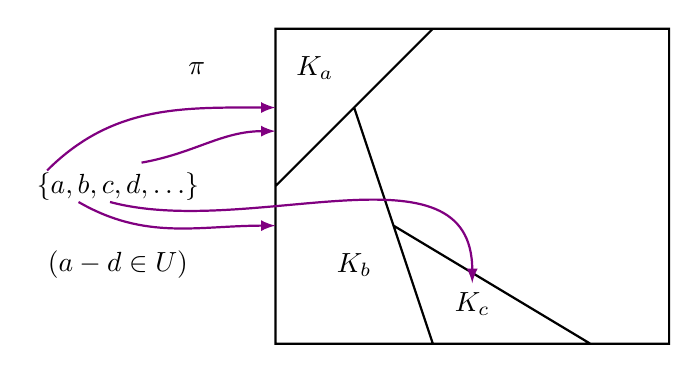
\begin{tikzpicture}
        \draw node at (3, 3.5) {$\pi$}
            node (set) at (2, 2) {$\{a,b,c,d,\ldots\}$}
            node [below of=set] {\normalsize$(a - d \in U)$}
            node (Ka) at (4.5, 3.5) {$K_a$}
            node (Kb) at (5, 1) {$K_b$}
            node (Kc) at (6.5, 0.5) {$K_c$}
            coordinate (a) at (1.1, 2.2)
            coordinate (b) at (1.5, 1.8)
            coordinate (c) at (1.9, 1.8)
            coordinate (d) at (2.3, 2.3);

        % \foreach \x in {1, 1.5, ..., 9}
        %     \foreach \y in {0, 0.5, ..., 4}
        %         \fill[black] (\x, \y) circle (1pt);

        % \foreach \pt in {a, b, c, d}
        %     \fill[red] (\pt) circle (1pt);

        \draw[thick] (4, 0) rectangle (9, 4)
            (4, 2) -- (6, 4)
            (5, 3) -- (6, 0)
            (5.5, 1.5) -- (8, 0);

        \draw[thick,violet,-latex] (a) to[out=45, in=180] (4, 3);
        \draw[thick,violet,-latex] (b) to[out=-30, in=180] (4, 1.5);
        \draw[thick,violet,-latex] (c) to[out=-15, in=90] (Kc);
        \draw[thick,violet,-latex] (d) to[out=10, in=180] (4, 2.7);
    \end{tikzpicture}

    \normalsize
    等价类:仿射子集(如何进一步描述其结构)

    商集:仿射子集构成的集合;商空间:商集上定义加法和数乘

    商映射:自然映射

    商空间的基与维数:两种方法
\end{figure}

\vspace{2ex}
\centerline{\heiti \Large 内容总结}

本讲我们首先从一般线性映射的逆出发引入矩阵的逆运算,并介绍了矩阵的逆的各种性质(注意没有加法性质),然后介绍了第一种逆矩阵求解的方法,即基于解方程的方法. 之后我们介绍了如何在线性空间的笛卡尔积和商集上定义运算使其构成新的空间——即积空间和商空间,并简单讨论了其中的映射,得到了一些启示,体验到了从定义线性空间的运算,到研究线性空间的结构(基和维数),最后利用线性映射同构等给出进一步结论的完整过程. 需要说明的一点是,尽管商空间看起来不是线性代数的重点,但实际上如果读者未来能学习到更多的数学课的话,与商空间类似的使用等价类定义的结构是很常见的,因此很有必要熟悉这其中的思想.

\vspace{2ex}
\centerline{\heiti \Large 习题}

\vspace{2ex}
{\kaishu 不管数学的任一分支是多么抽象,总有一天会应用在这实际世界上.}
\begin{flushright}
    \kaishu
    ——罗巴切夫斯基
\end{flushright}

\centerline{\heiti A组}
\begin{enumerate}
    \item 证明:若线性映射$\sigma \in \mathcal{L}(V_1,V_2)$可逆,则其逆映射唯一.

    \item 证明:\autoref{def:8:积空间} 中定义的线性空间的积构成一个线性空间.

    \item 证明以下两个命题:
          \begin{enumerate}
              \item 设$\varphi\in \mathcal{L}(V,\mathbf{F}),\enspace\varphi\neq 0$. 证明:$\dim V/(\ker\varphi)=1$;

              \item 设$U$是$V$的子空间且$\dim V/U=1$,则存在$\varphi\in \mathcal{L}(V,\mathbf{F})$使得$\ker\varphi=U$.
          \end{enumerate}
\end{enumerate}

\centerline{\heiti B组}
\begin{enumerate}
    \item 设$A$为$n$阶可逆矩阵,$A$的每行各元素之和都等于$k$,证明:$k \neq 0$且$A^{-1}$的每行各元素之和都等于$\vphantom{\cfrac{1}{k}}\dfrac{1}{k}$.

    \item 已知矩阵$A=\begin{pmatrix}1 & 2 & a  \\
               1 & 3 & 0  \\
               2 & 7 & -a\end{pmatrix}$可以通过初等列变换转化为矩阵$B=\begin{pmatrix}1  & a & 2 \\
               0  & 1 & 1 \\
               -1 & 1 & 1\end{pmatrix}$.
          \begin{enumerate}
              \item 求常数$a$;

              \item 求满足$AP=B$的可逆矩阵$P$.
          \end{enumerate}

    \item 设$A_1$和$A_2$均为$V$的仿射子集,证明:$A_1\cap A_2$是$V$的仿射子集或空集(可推广至任意交).

    \item 设$U$是$V$的子空间,$\Gamma:\mathcal{L}(V/U,W)\to \mathcal{L}(V,W)$定义为$\Gamma(S)=S\circ\pi$. 证明:
          \begin{enumerate}
              \item $\Gamma$是线性映射;

              \item $\Gamma$是单的;

              \item $\im\Gamma=\{T\in \mathcal{L}(V,W) \mid \forall u\in U,\enspace Tu=0\}$.
          \end{enumerate}
\end{enumerate}

\centerline{\heiti C组}
\begin{enumerate}
    \item 设 $A,B,C$ 为二阶复方阵,且 $A,B,C$ 在 $\mathbf{M}_2(\mathbf{C})$ 中线性无关. 证明:存在$z_1,z_2,z_3 \in \mathbf{C}$使得 $z_1A+z_2B+z_3C$ 为可逆矩阵.

    \item 设$v_1,\ldots,v_m\in V$. 令
          \[A=\{\lambda_1v_1+\cdots+\lambda_mv_m \mid \lambda_1,\ldots,\lambda_m\in\mathbf{F}\text{~且~}\lambda_1+\cdots+\lambda_m=1\}.\]
          证明:
          \begin{enumerate}
              \item $A$是$V$的仿射子集;

              \item $V$的每个包含$v_1,\ldots,v_m$的仿射子集均包含$A$;

              \item 存在某个$v\in V$和$V$的子空间$U$使得$A=v+U$且$\dim U\leqslant m-1$.
          \end{enumerate}
\end{enumerate}
